\documentclass[12pt,a4paper]{article}
\usepackage[utf8]{inputenc}
\usepackage[russian]{babel}
\usepackage[OT1]{fontenc}
\usepackage{graphicx}
\usepackage{calc}
\usepackage[margin=15mm]{geometry}
\usepackage{cmap}

% условие без картинки
\newcommand{\task}[2]{
\hrule
\hbox to \textwidth {%
     \vrule
\parbox[t]{0.04\textwidth}{\smallskip \centering #1}%
     \vrule%
\hfill%
     \parbox[t]{0.93\textwidth}{\smallskip #2 \smallskip}\hfill%
\vrule
}
\hrule
    \pagebreak[2]
}

\newlength{\h}
\newsavebox{\taskbox}
\newlength{\x}
\newsavebox{\pictbox}

% условие с картинкой (картинка выравнивается по центру)
\newcommand{\taskpic}[3]{
\savebox{\taskbox}{\parbox[t]{0.93\textwidth-4.3cm}{\smallskip #2 \smallskip}}
\savebox{\pictbox}{\parbox[t]{4cm}{\smallskip \centering
     \vspace{0pt} #3 \smallskip}}
\h=\ht\taskbox
\advance\h\dp\taskbox
\x=\ht\pictbox
\advance\x\dp\pictbox
\hrule
\hbox to \textwidth {%
\vrule\parbox[t][\maxof{\h}{\x}][t]{0.04\textwidth}{ \smallskip
     \centering #1 }\vrule%
\hfill\parbox[t][\maxof{\h}{\x}][t]{0.93\textwidth-4.3cm}{\smallskip #2
     \smallskip}\hfill\vrule%
\hfill\parbox[t][\maxof{\h}{\x}][c]{4cm}{\hfil #3 \hfil}\hfill\vrule
}
\hrule
\pagebreak[2]
}
\pagestyle{empty}
\graphicspath{ {images/} }

\begin{document}

\begin{center}
\begin{Large}
\textsc{ГЦФО. 9 класс. 2014/15.}
\end{Large}
\end{center}

\footnotesize

\task{41}{Поршень массы $M = 2$~кг может с трением скользить внутри вертикальной неподвижной трубы. Сначала поршень прикрепили внутри трубы к потолку пружиной жесткостью $k_1 = 20$~Н/м, длина которой в нерастянутом состоянии $l_1=60$~см. Поршень расположили на уровне середины трубы, отпустили, и он остался неподвижен. Затем опыт повторили, поменяв пружину - жесткость новой пружины стала $k_2 = 10$~Н/м, а длина в нерастянутом состоянии $l_2 = 20$~см. Удивительно, но поршень в середине трубы снова остался неподвижен. При каких значениях силы трения поршня о трубу это возможно? Влиянием воздуха пренебречь, $g = 10$~м/с$^2$.}
\taskpic{44}{Экспериментатор взял 4 одинаковых металлических стержня и собрал из них Y-образную фигуру. К концам фигуры экспериментатор присоединил 3 одинаковых больших металлических шара, имеющих температуру $t_1 = 0 ^\circ$C, $t_2 = 50 ^\circ$C и $t_3 = 100 ^\circ$C (см. рис.). Экспериментатор обеспечил хороший тепловой контакт стержней с шарами и другими стержнями. Через некоторое время он обнаружил, что первый шар нагрелся на $0{,}4^\circ$C. Какую температуру имели в этот момент два других шара? Считайте, что теплоемкость стержней пренебрежимо мала, а теплообмен с окружающей средой отсутствует. Мощность теплопередачи по стержню пропорциональна разности температур на его концах.}{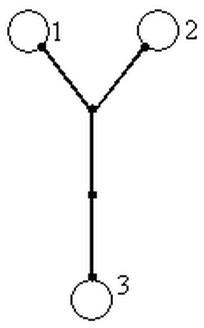
\includegraphics[width=2cm]{44}}
\taskpic{45}{Маленький шарик массы $m$, закрепленный на вертикальной пружине, расположили под столом с отверстием, в положении равновесия шарик находится посередине отверстия. Обнаружилось, что если шарик отклонить вниз на произвольное расстояние и отпустить, он колеблется вокруг положения равновесия с периодом $T_0$. Над отверстием поставили тело массой $m$ (см. рис.) и снова вывели шарик из положения равновесия. Определить период колебаний системы, если известно, что максимальная скорость шарика $v_m$. Шарик и тело соударяются абсолютно упруго; тело, подскакивая, движется строго вертикально. Сопротивлением воздуха пренебречь, ускорение свободного падения~$g$.}{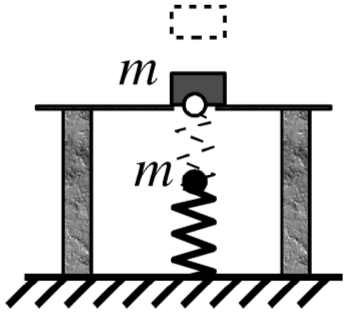
\includegraphics[width=4cm]{45}}
\taskpic{46}{Длинный однородный брусок с поперечным сечением в виде прямоугольника со сторонами $a \neq b$ подвешен на двух вертикальных нитях, прикрепленных к одному из ребер, над сосудом, в который наливают воду. Когда в сосуд налили некоторое количество воды, два ребра бруска оказались точно на поверхности воды (вид сбоку, со стороны вышеупомянутого поперечного сечения, показан на рисунке). Найдите плотность материала, из которого сделан брусок. Плотность воды $\rho = 1$~г/см$^3$.\\
Примечание: центр масс однородного треугольника расположен на пересечении его медиан.}{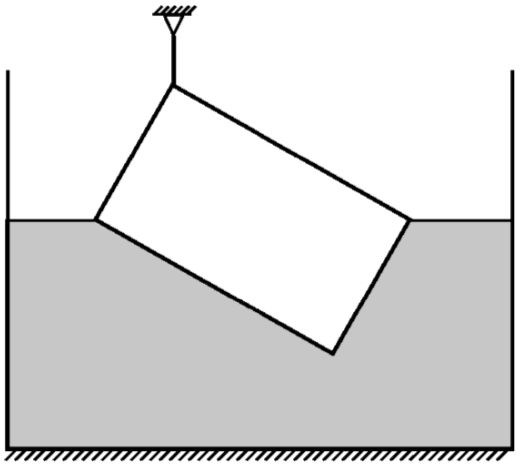
\includegraphics[width=4cm]{46}}
\taskpic[65mm]{47}{В <<черном ящике>> находится схема, состоящая из последовательно соединенных идеальной батарейки с напряжением $U_0 = 3{,}3$~В и резистора сопротивлением $R_0 = 1500$~Ом (рисунок слева). При попытке изготовить второй такой же <<черный ящик>> оказалось, что батареек с нужным напряжением 3{,}3~В в лаборатории больше нет, зато есть другая идеальная батарейка с напряжением $U_1 = 5$~В. По этой причине решили собрать схему, состоящую из имеющейся батарейки и двух резисторов, соединив эти элементы так, как изображено на рисунке справа. Найдите, какими должны быть сопротивления резисторов $R_1$ и $R_2$ для того, чтобы два этих <<черных ящика>> оказались эквивалентными друг другу.}{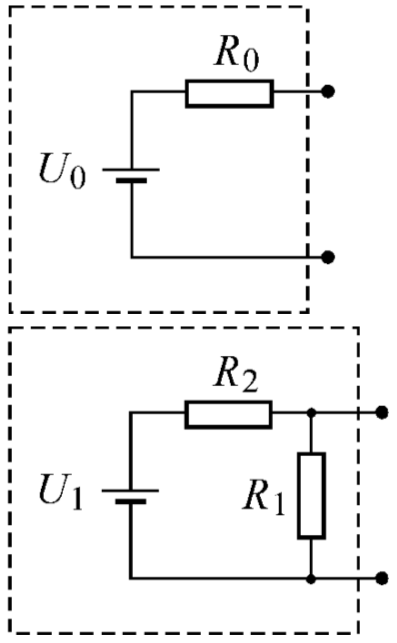
\includegraphics[width=6cm]{47}}
\task{48}{Для изготовления нагревательной спирали кипятильника взяли проволоку длиной $l_1$. После подключения этого кипятильника к источнику напряжения с малым внутренним сопротивлением на нагревание некоторой массы воды в калориметре на $50^\circ$C было затрачено время $\tau_1 = 2$~минуты. Затем проволоку, из которой была сделана спираль кипятильника, расплавили и изготовили из расплава новую проволоку длиной $l_2 = 2l_1$. Из новой проволоки сделали другую спираль для кипятильника, опустили его в другой калориметр с другим количеством воды, и подключили кипятильник к тому же источнику напряжения. На нагревание воды на $50^\circ$C во втором калориметре было потрачено время $\tau_2 = 12$~минут. Во сколько раз масса воды во втором калориметре отличается от массы воды в первом калориметре? Считайте, что потерь теплоты при нагревании воды не происходит, теплоемкости калориметров пренебрежимо малы, а плотность и проводимость металла после переплавки остаются прежними.}
\end{document}
